\documentclass[
Karos,
%Loesung,
%Punkte
]{pruefung}

\renewcommand{\Pruefungsfach}{\textbf{Prüfungsfach: Mathematik 2}}
\renewcommand{\Semester}{\textbf{Wintersemester 23/24}}
\renewcommand{\Studiengaenge}{\textbf{Studiengänge: SWB/TIB/IEP}}
\renewcommand{\Fachnummern}{\textbf{Prüfungsnummer: IT 105  20 03 / IT 105 20 13}}
\renewcommand{\Dauer}{\textbf{Zeit: 90 Minuten}}
\renewcommand{\Dozenten}{\textbf{Dozent: Prof. Dr. Jürgen Koch}}

\renewcommand{\Hilfsmittel}{
\textbf{Manuskript\newline
 Literatur\newline
Taschenrechner Casio FX-87DE Plus / Casio FX-87DE Plus 2nd edition}
}
\renewcommand{\Hinweise}{
\textbf{Bearbeiten Sie die Aufgaben ausschließlich auf diesen Prüfungsblättern.
\newline
Begründen Sie alle Lösungsschritte.}
}

\begin{document}
\begin{Aufgabe}[10]
Hinweis: Alle Teilaufgaben können unabhängig voneinander bearbeitet werden.

\begin{enumerate}
	\item
		Ordnen Sie den Differenzialgleichungen die Richtungsfelder zu:
		
		\begin{tabular}{p{0.25\textwidth}p{0.25\textwidth}p{0.25\textwidth}p{0.25\textwidth}}
			(A) $\displaystyle y' = \frac{x}{y}$ &
			(B) $\displaystyle y' = \frac{y}{x}$ &
			(C) $\displaystyle y' = -\frac{x}{y}$ &
			(D) $\displaystyle y' = -\frac{y}{x}$ \\
		\end{tabular}
		
		\begin{tabular}{llll}
			\ifLoesung
			( {\textcolor{red}C} ) &
			\else
			( \quad ) &
			\fi
			\hspace*{-10mm} \raisebox{-0.8\height}{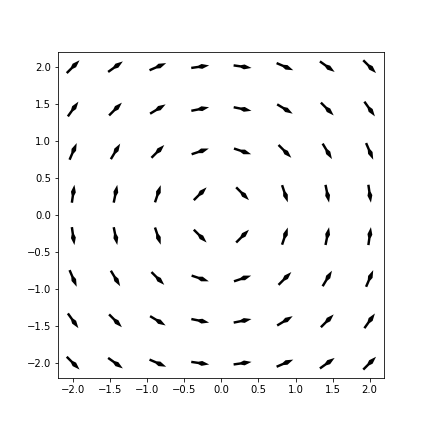
\includegraphics[width=0.4\textwidth]{../M2_IT/m2_it_ws_23_kurzaufgaben_richtungsfeld_3.png}} &
			\ifLoesung
			( {\textcolor{red}D} ) &
			\else
			( \quad ) &
			\fi
			\hspace*{-10mm} \raisebox{-0.8\height}{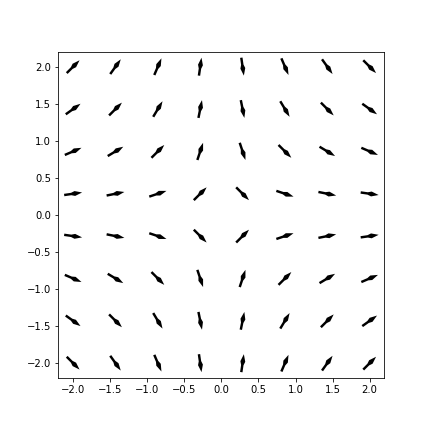
\includegraphics[width=0.4\textwidth]{../M2_IT/m2_it_ws_23_kurzaufgaben_richtungsfeld_4.png}}  \\
			\ifLoesung
			( {\textcolor{red}B} ) &
			\else
			( \quad ) &
			\fi
			\hspace*{-10mm} \raisebox{-0.8\height}{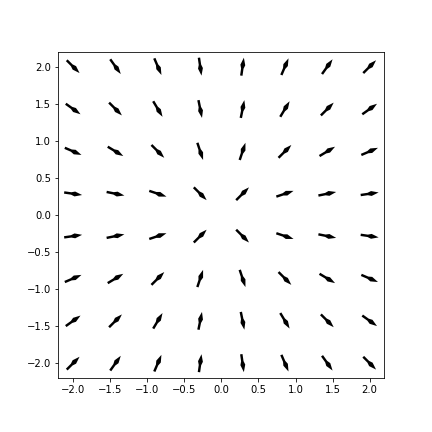
\includegraphics[width=0.4\textwidth]{../M2_IT/m2_it_ws_23_kurzaufgaben_richtungsfeld_2.png}} &
			\ifLoesung
			( {\textcolor{red}A} ) &
			\else
			( \quad ) &
			\fi
			\hspace*{-10mm} \raisebox{-0.8\height}{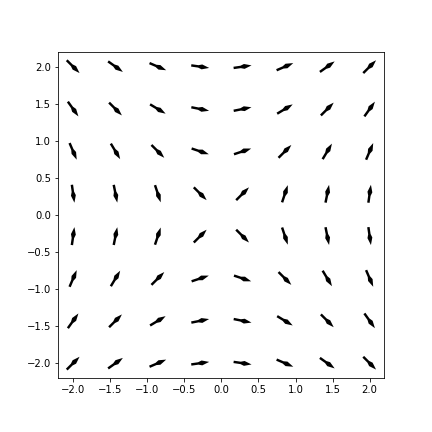
\includegraphics[width=0.4\textwidth]{../M2_IT/m2_it_ws_23_kurzaufgaben_richtungsfeld_1.png}}  \\
		\end{tabular}
		
		\ifLoesung
		\mbox{}\hfill\Punkte{2 P}\\
		\fi	
		
		\pagebreak
	\item
		Bestimmen Sie die allgemeine Lösung der Differenzialgleichung
		\[
			y'(x) = 3 \, x^2 \, y \, .
		\]
		
		\Loesung{10cm}{
			Separation:
			\hfill\Punkte{1 P}
			\[
				\frac{\mathrm{d} \, y}{\mathrm{d} \, x} = 3 \, x^2  \, y 
				\quad \Longrightarrow \quad
				\frac{1}{y} \, \mathrm{d} \, y = 3 \, x^2 \, \mathrm{d} \, x \, .
			\]
			Integration:
			\hfill\Punkte{1 P}
			\[
				\int \frac{1}{y} \, \mathrm{d} \, y = \int 3 \, x^2 \, \mathrm{d} \, x 
				\quad \Longrightarrow \quad
				\ln \left| y \right| = x^3 + C_1, \quad C_1 \in \mathbb{R} \, .
			\]
			Nach $y$ auflösen:
			\hfill\Punkte{1 P}
			\[
				\left| y \right|  = \e^{x^3 + C_1}
				\quad \Longrightarrow \quad
				y = \pm \e^{x^3 + C_1} = \pm \e^C_1 \, \e^{x^3} = C_2 \, \e^{x^3}, \quad C_2 \in \mathbb{R} \, .
			\]
		}
		
	\item
		Berechnen Sie für die Lösung des Anfangswertproblems
		\[
			y'(x) = \frac{y}{1 + x^2}, \quad y(1) = 3 \, ,
		\]
		einen Näherungswert, indem Sie einen Schritt mit dem Euler-Polygonzugverfahren mit der Schrittweite $h=0.2$ durchführen.
		
		\Loesung{}{
			Euler-Polygonzugverfahren:
			\[
			x_1 = x_0 + h = 1.2, 
			\quad
			\tilde{y}_1 = 
			\tilde{y}_0 + h \cdot  \frac{\tilde{y}_0 }{1 + x_0^2} = 
			3 + 0.2 \cdot  \frac{3}{1 + 1^2} = 3.3 \, .
			\hfill\Punkte{2 P}
			\]
		}
		
		\newpage
		
	\item
		Beurteilen Sie den folgenden Dialog mit ChatGPT 3.5.
		Sind die Berechnungen und die Behauptungen von ChatGPT korrekt?
		 
		 \vspace*{2ex}
		 
		 \textbf{You}
		 
		Bitte erstelle ein Beispiel für ein lineares Differenzengleichungssystem mit zwei Unbekannten, das asymptotisch stabil ist.
		
		\vspace*{2ex}
		
		\textbf{ChatGPT}
		
		Betrachten wir das folgende lineare Differenzengleichungssystem mit zwei Unbekannten:
		\[
			\begin{array}{lcl}
				x_{k+1} & = & 0.8 \, x_k + 0.2 \, y_k \\
				y_{k+1} & = & 0.4 \, x_k + 0.6 \, y_k
			\end{array}
		\]
		Die obigen Gleichungen können in Matrixform geschrieben werden als:
		\[
			\left(
				\begin{array}{c}
					x_{k+1} \\
					y_{k+1}
				\end{array}
			\right)
			= 
			\left(
			\begin{array}{cc}
				0.8 & 0.2 \\
				0.4 & 0.6
			\end{array}
			\right)
			\left(
			\begin{array}{c}
				x_{k} \\
				y_{k}
			\end{array}
			\right), \mbox{ mit der Matrix }
			\mathbf{A} =
			\left(
			\begin{array}{cc}
				0.8 & 0.2 \\
				0.4 & 0.6
			\end{array}
			\right)
		\]
		Die Matrix $\mathbf{A}$ ist die Übertragungsmatrix des Systems.
		Um die asymptotische Stabilität zu überprüfen, betrachten wir die Eigenwerte dieser Matrix.
		Die Eigenwerte $\lambda$ können durch das Lösen der charakteristischen Gleichung gefunden werden:
		\[
			\left|
				\begin{array}{cc}
					0.8 - \lambda & 0.2 \\ 
					0.4 & 0.6 - \lambda
				\end{array}
			\right| = 0
			\quad \Longleftrightarrow \quad
			(0.8 - \lambda)(0.6 - \lambda) -0.2 \cdot 0.4 = 0
			\quad \Longleftrightarrow \quad
			\lambda^2 - 1.4 \, \lambda + 0.4 = 0
		\]
		Die Lösungen dieser quadratischen Gleichung sind $\lambda_1=1$ und $\lambda_2=0.4$.
		Beide Eigenwerte haben Beträge kleiner als $1$, was darauf hinweist, dass  das System asymptotisch stabil ist.
		In diesem Beispiel konvergieren die Lösungen für $x_k$ und $y_k$ gegen Null, was auf eine asymptotische Stabilität hinweist.  
		
		\Loesung{}{
			Die Berechnungen sind korrekt.
			Das System ist jedoch nicht asymptotisch stabil, denn der Betrag des Eigenwerts $\lambda_1 = 1$ ist nicht echt kleiner $1$.
			Deshalb konvergieren auch nicht alle Lösungen gegen Null.
			Beispielsweise ist $x_0=1$ und $y_0=1$ ein Fixpunkt. 
			\hfill\Punkte{3 P}
		}
			
	\end{enumerate}
	
\end{Aufgabe}

\newpage

\endinput
\begin{Aufgabe}[9]
	Bestimmen Sie die allgemeine reelle Lösung der Differenzialgleichung
	\[
		y''(x)+ 4 \, y(x) = 8 \, \cos(2 \, x) - 4 \, \sin(2 \, x) \, .
	\]
	
	\Loesung{}{
		Charakteristische Gleichung der homogenen  Differenzialgleichung:
		\hfill\Punkte{2 P}
		\[
			\lambda^2 + 4 = 0
			\quad \Longrightarrow \quad
			\lambda^2 = -4 
			\quad \Longrightarrow \quad
			\lambda = \pm 2 \, \mbox{i} \, .
		\]
		Allgemeine Lösung der homogenen  Differenzialgleichung:
		\hfill\Punkte{1 P}
		\[
			y_h(x) = C_1 \, \cos(2 \, x) + C_2 \, \sin(2 \, x) \, .
		\]
		Ansatz für partikuläre Lösung mit Resonanz:
		\hfill\Punkte{1 P}
		\[
			y_p(x) = x ( A \, \cos(2 \, x) + B \, \sin(2 \, x) ) \, .
		\]
		Erste Ableitung:
		\hfill\Punkte{1 P}
		\[
			y'_p(x) = A \, \cos(2 \, x) + B \, \sin(2 \, x) )+x \, ( - 2\, A \, \sin(2 \, x) + 2 \, B \, \cos(2 \, x) ) \, .
		\]
		Zweite Ableitung:
		\hfill\Punkte{1 P}
		\[
			y''_p(x) = -2 \, A \, \sin(2 \, x) + 2 \, B \, \cos(2 \, x) ) - 2\, A \, \sin(2 \, x) + 2 \, B \, \cos(2 \, x) + x \, ( - 4\, A \, \cos(2 \, x) - 4 \, B \, \sin(2 \, x) )\, .
		\]
		In Differenzialgleichung einsetzen:
		\hfill\Punkte{1 P}
		\begin{eqnarray*}
			\underbrace{-4 \, A \, \sin(2 \, x) + 4 \, B \, \cos(2 \, x) + x \, ( - 4\, A \, \cos(2 \, x) - 4 \, B \, \sin(2 \, x) )}_{\displaystyle y''(x)} & + & 4 \, \underbrace{x ( A \, \cos(2 \, x) + B \, \sin(2 \, x)) }_{\displaystyle y(x)} \\
			& = & 8 \, \cos(2 \, x) - 4 \, \sin(2 \, x) \, .
		\end{eqnarray*}
		Koeffizientenvergleich:
		\hfill\Punkte{1 P}
		\[
			A = 1, \quad B = 2 \, .
		\]
		Allgemeine Lösung:
		\hfill\Punkte{1 P}
		\[
			y(x) = y_h(x) + y_p(x) = C_1 \, \cos(2 \, x) + C_2 \, \sin(2 \, x) + x ( \cos(2 \, x) + 2 \, \sin(2 \, x) ) \, .
		\]
	}
	
	\ifLoesung
	\else
	\newpage
	
	\Loesung{}{}
	\fi
	
\end{Aufgabe}

\newpage

\endinput
\begin{Aufgabe}[10]% Siehe SS 16
	Bestimmen Sie die allgemeine reelle Lösung des Differenzialgleichungssystems
	\[
	\begin{array}{ccrcrcr}
		\dot{x}_1 & = & -2 \, x_1 & + & 3 \, x_2 & + & 6 \, \e^{-2 \, t} \, ,\\
		\dot{x}_2 & = &  2 \, x_1 &  + & 3 \, x_2 & .   &  \\
	\end{array}
	\]
	
	\Loesung{}{
		Matrixform:
		\hfill\Punkte{1 P}
		\[
		\dot{\mathbf{x}}
		=
		\left(
		\begin{array}{rr}
			-2 & 3\\
			2 &  3\\
		\end{array}
		\right)
		\mathbf{x} +
		\left(
		\begin{array}{c}
			 6 \, \e^{-2 \, t}\\
			0\\
		\end{array}
		\right)
		\, .
		\]
		Eigenwerte:
		\hfill\Punkte{2 P}
		\[
		\left|
		\begin{array}{cc}
			-2-\lambda &            3\\
			2                & 3 - \lambda\\
		\end{array}
		\right|
		=(-2-\lambda)(3-\lambda)-3 \cdot 2 = \lambda^2-\lambda-12 = 0
		\, \Longrightarrow \,
		\lambda_{1,2} = \frac{1\pm\sqrt{1+48}}{2} = 4 | -3 \, .
		\]
		Eigenvektor $\mathbf{v}_1$ zu $\lambda_1=4$:
		\hfill\Punkte{1 P}
		\[
		\left(
		\begin{array}{cc}
			-2-4 &                 3\\
			2                     & 3-4\\
		\end{array}
		\right)
		\mathbf{v}_1
		=
		\left(
		\begin{array}{rr}
			-6 &  3\\
		 2  & -1\\
		\end{array}
		\right)
		\mathbf{v}_1
		= \mathbf{0}
		\quad \Longrightarrow \quad
		\mathbf{v}_1
		=
		\left(
		\begin{array}{c}
			1\\
			2\\
		\end{array}
		\right) \, .
		\]
		Eigenvektor $\mathbf{v}_2$ zu $\lambda_2=-3$:
		\hfill\Punkte{1 P}
		\[
		\left(
		\begin{array}{cc}
			-2+3 &                 3\\
			2                     & 3+3\\
		\end{array}
		\right)
		\mathbf{v}_2
		=
		\left(
		\begin{array}{cc}
			1 &  3\\
			2  & 6\\
		\end{array}
		\right)
		\mathbf{v}_2
		= \mathbf{0}
		\quad \Longrightarrow \quad
		\mathbf{v}_2
		=
		\left(
		\begin{array}{r}
			3\\
			-1\\
		\end{array}
		\right) \, .
		\]
		Allgemeine reelle Lösung des homogenen Differenzialgleichungssystems:
		\hfill\Punkte{1 P}
		\[
		\mathbf{x}_h
		= C_1 \, \e^{4 \, t}\
		\left(
		\begin{array}{c}
			1\\
			2\\
		\end{array}
		\right)
		+ C_2 \, \e^{- 3 \, t}
		\left(
		\begin{array}{r}
		 3\\
			-1\\
		\end{array}
		\right),
		\quad C_1, C_2\in \mathbb{R} \, .
		\]
	}
	
	\newpage
	
	\Loesung{}{
		Ansatz für partikuläre Lösung ohne Resonanz:
		\hfill\Punkte{1 P}
		\[
			\mathbf{x}_p
			= \e^{- 2 \, t}\
			\left(
			\begin{array}{c}
				A\\
				B\\
			\end{array}
			\right) \, .
		\]
		Ableitung in Differenzialgleichungssystem eingesetzt:
		\hfill\Punkte{1 P}
		\[
			-2 \, \e^{- 2 \, t}\
			\left(
			\begin{array}{c}
				A\\
				B\\
			\end{array}
			\right)
			=
			\left(
			\begin{array}{rr}
				-2 & 3\\
				2 &  3\\
			\end{array}
			\right)
			\e^{- 2 \, t}\
			\left(
			\begin{array}{c}
				A\\
				B\\
			\end{array}
			\right) +
			\left(
			\begin{array}{c}
				6 \, \e^{-2 \, t}\\
				0\\
			\end{array}
			\right)
			\, .
		\]
		Lineares Gleichungssystem:
		\hfill\Punkte{1 P}
		\[
			\begin{array}{rcrcrcr}
				-2 \, A & = & -2 \, A & + & 3 \, B & + & 6 \\
				-2 \, B & = &   2 \, A & + & 3 \, B &    & \\
			\end{array}
			\quad \Longrightarrow \quad
			B = -2, \, A = 5 \, .
		\]
		Allgemeine reelle Lösung des Differenzialgleichungssystems:
		\hfill\Punkte{1 P}
		\[
			\mathbf{x} = \mathbf{x}_h + \mathbf{x}_p
			= C_1 \, \e^{4 \, t}\
			\left(
			\begin{array}{c}
				1\\
				2\\
			\end{array}
			\right)
			+ C_2 \, \e^{- 3 \, t}
			\left(
			\begin{array}{r}
				3\\
				-1\\
			\end{array}
			\right) +
			e^{- 2 \, t}
			\left(
			\begin{array}{r}
				 5\\
				-2\\
			\end{array}
			\right),
			\quad C_1, C_2\in \mathbb{R} \, .
		\]
	}
	
\end{Aufgabe}

\newpage

\endinput
\begin{Aufgabe}[8] 
	Eine Differenzengleichung erster Ordnung ist gegeben durch
	\[
		x_{k+1} = 1.05 \, x_k - 1, \quad x_0 = 10, \quad k = 0,1,2,3,\ldots . 
	\]
	\begin{enumerate}
		\item
			Geben Sie die Zahlenwerte von $x_1$ und $x_2$ an.
		\item
		  	Bestimmen Sie die Lösung der Differenzengleichung.
		 \item
		 	Für welche Indizes $k$ ist $x_k < 0$?  
	\end{enumerate}
	
	\Loesung{}{
		\begin{enumerate}
			\item
				Zahlenwerte:
				\hfill\Punkte{1 P}
				\[
					x_0 = 1.05 \cdot 10 - 1 = 9.5, \quad x_1 = 1.05 \cdot 9.5 - 1 = 8.975
				\]
			\item
				Lösungsformel:
				\hfill\Punkte{1 P}
				\[
					x_{k+1} = \lambda \, x_k + r_k
					\quad \Longrightarrow \quad
					x_k = \lambda^k \cdot x_0 + \sum_{l=0}^{k-1} \lambda^{k-1-l} r_l \, .
				\]
				$\lambda = 1.05$, $r_k = -1$, $x_0 = 1$:
				\hfill\Punkte{1 P}
				\[
					x_k = 1.05^k \cdot 10 + \sum_{l=0}^{k-1}1.05^{k-1-l} \cdot (-1) \, .
				\]
				Geometrische Reihe:
				\hfill\Punkte{1 P}
				\[
					x_k =
					1.05^k \cdot 10 - \frac{1 - 1.05^k}{1 - 1.05} \, .
				\]
				Vereinfachung:
				\hfill\Punkte{1 P}
				\[
					x_k =
					10 \cdot 1.05^k  - \frac{1 - 1.05^k}{- 0.05} =
					10 \cdot 1.05^k  + 20 - 20 \cdot 1.05^k =
					- 10 \cdot 1.05^k  + 20\, .
				\]
			\item
				Bedingung $x_k < 0$:
				\hfill\Punkte{1 P}
				\[
					- 10 \cdot 1.05^k  + 20 < 0
					\quad \Longleftrightarrow \quad
					20 < 10 \cdot 1.05^k
					\quad \Longleftrightarrow \quad
					2 < 1.05^k \, .
				\]
				Nach $k$ auflösen:
				\hfill\Punkte{1 P}
				\[
					\ln(2) < \ln\left((1.05)^k\right)
					\quad \Longleftrightarrow \quad
					\ln(2) < k \, \ln(1.05)
					\quad \Longleftrightarrow \quad
					k > \frac{\ln(2)}{\ln(1.05)} \approx 14.2
				\]
				Ab $k = 15$ sind alle Folgenglieder negativ.
				\hfill\Punkte{1 P}
		\end{enumerate}
	}
	
	\newpage
	
	\Loesung{}{
		Alternative Lösung für \textbf{b)}
		\par
		\vspace*{1cm}
		\par
		Homogene Lösung:
		\[
			x_{k+1} -1.05 \, x_k = 0
			\quad \Longrightarrow \quad
			\lambda - 1.05 = 0
			\quad \Longrightarrow \quad
			\lambda = 1.05
			\quad \Longrightarrow \quad
			x_k^h = C \cdot 1.05^k \, .
		\]
		Partikuläre Lösung
		\[
			x_k^p = A
			\quad \Longrightarrow \quad
			A - 1.05 \, A = - 1
			\quad \Longrightarrow \quad
			A ( 1 - 1.05 ) = -1
			\quad \Longrightarrow \quad
			A = \frac{-1}{-0.05} = 20 \, .
		\]
		Allgemeine Lösung:
		\[
			x_k = x_k^h + x_k^p = C \cdot 1.05^k + 20 \, .
		\]
		Anfangswert $x_0 = 10$: 
		\[
			k = 0: \quad 
			x_0 = C \cdot 1.05^0 + 20 
			\quad \Longrightarrow \quad
			10 = C + 20
			\quad \Longrightarrow \quad
			C = -10 \, .
		\]
		Ergebnis:
		\[
			x_k = -10 \cdot 1.05^k + 20 \, .
		\]
	}
	
\end{Aufgabe} 

\newpage

\endinput
\begin{Aufgabe}[9]% SS 18
	Gegeben ist die Funktion $f$ mit
	\[
		f(x) = \e^{-x^2} \, .
	\]
	\begin{enumerate}
		\item
			Entwickeln Sie die Funktion $f$ in eine Potenzreihe um die Entwicklungsstelle $x_0 = 0$.
			Für welche $x$ Werte konvergiert die Reihe?
		\item
			Berechnen Sie einen Näherungswert $\tilde{I}$ für das bestimmte Integral
			\[
				I = \int_0^{1} \, f(x) \, \mbox{d} \, x
			\]
			mithilfe der Potenzreihe mit den Gliedern bis zur Ordnung $4$.
			Schätzen Sie die maximale Abweichung 
			\mbox{$| I - \tilde{I} |$}
			des Näherungswertes $\tilde{I}$ vom exakten Wert $I$ mit dem Leibniz-Kriterium ab.
		\item
			Geben Sie eine Formel für $f^{(n)}(0)$ an, d.h. für die $n$-te Ableitung der Funktion $f$ an der Stelle $x=0$.
			Unterscheiden Sie dabei die Fälle für gerades und ungerades $k$.
	\end{enumerate}
	
	\Loesung{}{
		\begin{enumerate}
			\item
			Potenzreihenentwicklung konvergiert für alle reellen Zahlen
			\hfill\Punkte{2 P}
			\[
			\mbox{e}^x = \sum_{k=0}^\infty  \frac{x^k}{k \, !} = 1 + x + \tfrac{x^2}{2!} + \tfrac{x^3}{3!} + \ldots
			\quad \Longrightarrow \quad
			f(x) = \sum_{k=0}^\infty  \frac{(-x^2)^k}{k \, !}  = 1 - x^2 + \tfrac{x^4}{2} - \tfrac{x^6}{6} \pm \ldots
			\]
			\item
			Gliedweise Integration der Potenzreihenentwicklung 
			\hfill\Punkte{3 P}
			\[
			\tilde{I}
			= \int_0^1 \, 1 - x^2 + \tfrac{x^4}{2}  \, \mbox{d} \, x
			= \left[ x - \tfrac{x^3}{3} + \tfrac{x^5}{10} \right]_0^1
			= 1 - \tfrac{1}{3} + \tfrac{1}{10} = \tfrac{23}{30} \, .
			\]
			Abschätzung der maximalen Abweichung mit der Leibniz-Kriterium für alternierende Reihen:
			\hfill\Punkte{2 P}
			\begin{align*}
				| I - \tilde{I} |
				& = \left| \int_0^1 f(x)\mbox{d} \, x - \int_0^1 1-x^2+\frac{x^4}{2}\, \mbox{d} \, x \right|
				= \left| \int_0^1 f(x) - \left(1-x^2+\frac{x^4}{2}\right) \, \mbox{d}\, x \right|\\
				& \leq \int_0^1 \left|f(x) - \left(1-x^2+\frac{x^4}{2}\right)\right| \, \mbox{d}\, x 
				\leq \int_0^1 \left|-\frac{x^6}{6} \right| \, \mbox{d} \, x 
				= \left[ \frac{x^7}{7 \cdot 6} \right]_0^1
				= \frac{1}{42} \, .
			\end{align*}
			\item
			Formel für die Ableitung
			\hfill\Punkte{2 P}
			\[
				f(x) = \sum_{k=0}^\infty \frac{(-1)^{k}}{k \, !} x^{2 \, k} 
				\quad \Longrightarrow \quad 
				\frac{f^{(2 \, k)}(0)}{(2 \, k)!} = \frac{(-1)^{k}}{k \, !}
				\quad \Longrightarrow \quad 
				\frac{f^{(n)}(0)}{n!} = \frac{(-1)^{n/2}}{(n/2) \, !} \mbox{ für $n$ gerade} \, .
			\]
			Für ungerade $n$ ist die $n$-te Ableitung null.
		\end{enumerate}
	}
	
	\newpage
	
	\ifLoesung
	\else
	\Loesung{}{}
	\newpage
	\fi	
	
\end{Aufgabe}

\newpage

\endinput
\begin{Aufgabe}[8]
	Gegeben ist die periodische Funktion $f$, mit
	\[
		f(t) = t^2 \mbox{ für } t \in [-2, 2), \quad f(t + 4) = f(t) \, .
	\]
	\begin{enumerate}
		\item
			Skizzieren Sie die Funktion $f$ für $t \in [-2, 10]$.
		\item
			Bestimmen Sie den Mittelwert $m$ der Funktion $f$.
		\item
			An welchen Stellen tritt bei der Funktion $f$ das Gibbsche Phänomen auf?
		\item
			Im folgenden bezeichnen $a_k$, $b_k$ die reellen und $c_k$ die komplexen Fourier-Koeffizienten der Funktion $f$.
			Welche der folgenden Aussagen ist wahr und welche ist falsch?
			
			\ifLoesung 
			\begin{tabular}{p{0.3\textwidth}p{0.2\textwidth}p{0.2\textwidth}}
				Alle $a_k$ sind null                & $\square$ wahr               & {\textcolor{red}X} falsch\\
				Alle $b_k$ sind null                & {\textcolor{red}X} wahr  &              $\square$ falsch\\
				Alle $c_k$ sind reell               &  {\textcolor{red}X} wahr &              $\square$ falsch\\
				Alle $c_k$ sind rein imaginär & $\square$ wahr              & {\textcolor{red}X} falsch\\
			\end{tabular}
			\hfill\Punkte{2 P}
			\else
			\begin{tabular}{p{0.3\textwidth}p{0.2\textwidth}p{0.2\textwidth}}
				Alle $a_k$ sind null                 & $\square$ wahr & $\square$ falsch\\
				Alle $b_k$ sind null                 & $\square$ wahr & $\square$ falsch\\
				Alle $c_k$ sind reell                & $\square$ wahr & $\square$ falsch\\
				Alle $c_k$ sind rein imaginär & $\square$ wahr & $\square$ falsch\\
			\end{tabular}
			\fi
	\end{enumerate}
	
	\begin{tikzpicture}[xscale=1.0,yscale=1.0]
		\draw[line width=0.25pt,step=0.5cm,color=lightgray] (-4.0,-6.0) grid(13.5cm,6.0cm);
		\draw[->,thick] (-3.5, 0.0) -- (13.0, 0.0) node[below=1mm] {$t$};
		\draw[->,thick] ( 0.0,-5.5) -- ( 0.0,5.5) node[left]  {$f$};
		\foreach \i in {-5,-4,-3,-2,-1,1,2,3,4,5} {
			\draw[thick] (0.1,\i) -- (-0.1,\i) node[left] {$\i$};
		}
		\foreach \i in {-3,-2,-1,1,2,3,4,5,6,7,8,9,10,11,12} {
			\draw[thick] (\i,0.1) -- (\i,-0.1) node[below] {$\i$};
		}
		
		\ifLoesung
		\draw[ultra thick, smooth, domain=-2:2,color=red] plot (\x,{\x*\x});
		\draw[ultra thick, smooth, domain=2:6,color=red] plot (\x,{(\x-4)*(\x-4)});
		\draw[ultra thick, smooth, domain=6:10,color=red] plot (\x,{(\x-8)*(\x-8)}) ;
		\fi
	\end{tikzpicture}
	
	\Loesung{}{
		\begin{enumerate}[series=fourierreihen_loesung]
			\item
				Skizze:
				\hfill\Punkte{2 P}
		\end{enumerate}
	}
	
	\newpage
	
	\Loesung{}{
		\begin{enumerate}[resume=fourierreihen_loesung]
			\item
				Mittelwert:
				\hfill\Punkte{3 P}
				\[
				m
				= \frac{1}{T} \int_{-T/2}^{T/2} f(t) \, \mathrm{d} \, t
				= \frac{1}{4} \int_{-2}^{2} t^2 \, \mathrm{d} \, t
				= \frac{1}{4} \left[ \frac{t^3}{3} \right]_{-2}^{2} 
				= \frac{16}{12}
				= \frac{4}{3} \, .
				\]
				\item
				Die Funktion $f$ ist stetig, deshalb tritt das Gibbsche Phänomen nicht auf.
				\hfill\Punkte{1 P}
		\end{enumerate}
	}
	
\end{Aufgabe}

\newpage

\endinput
\end{document}
